\chapter{Validación, verificación, y evaluación}\label{chap:validation}

Este capítulo verificará que la solución propuesta cumple con todos los
requisitos especificados en el \chapterref{analysis}, y está dividido en dos
secciones. La primera (\sectionref{tests}), contendrá la verificación y
validación de software, mientras que la segunda (\sectionref{evaluation})
contendrá una evaluación del sistema, comparándolo con otras herramientas
existentes.

\section{Verificación y Validación}\label{sec:tests}

En ingeniería de software, la verificación y validación de software es el
proceso de comprobación de que el sistema cumple con los requisitos establecidos
y la función para la que se diseñó \parencite{verification-validation}. La
\figureref{tests} muestra un resumen de este proceso.

\drawiosvgfigure[0.75]{tests}{Resumen de la verificación y validación de software}

Como se explicó en el \chapterref{analysis}, el cliente establece sus
necesidades y lo que espera del producto, definiendo los requisitos de software.
A partir de estos requisitos, el analista se encarga de definir los requisitos
de software.

La verificación de software (\subsectionref{verification}) se encarga de,
durante el desarrollo del sistema, comprobar que los productos de una fase de
desarrollo cumplen con los requisitos establecidos al inicio de la fase; es
decir, comprobar que se está desarrollando el sistema correctamente. Por otro
lado, la validación de software (\subsectionref{validation}) se encarga de, al
final del desarrollo del sistema, comprobar que cumple con los requisitos
establecidos por el cliente; es decir, comprobar que se ha desarrollado el
sistema correcto. \parencite{verification-validation}

\printtesttemplate

\subsection{Verificación}\label{subsec:verification}

Esta sección contiene las pruebas de verificación realizadas. Estas pruebas,
además de verificar que se cumplen los requisitos de software, también verifican
que el resultado del sistema desarrollado es el correcto en todos los casos
probados. Después de realizar estas pruebas, se ha realizado una matriz de
trazabilidad (\tableref{traceability-rs-vet}) para comprobar que todos los
requisitos de software están cubiertos por al menos una prueba de verificación.

\begin{testCase}{VET}{ISA}
    {El sistema está instalado.} % Precondición
    {Se obtiene el código compilado correspondiente al programa introducido.} % Postcondición
    {Verificar que el sistema puede compilar \glspl{program} en una \gls{ISA}.} % Descripción
    {OK} % Evaluación
    {FN-compilar-instrucciones, FN-directivas, FN-secciones, FN-ISA,
    FN-num-etiquetas, FN-referencias, NF-ISA, NF-def-instrucciones, NF-sintaxis} % Origen
    \begin{enumerate}[leftmargin=*, topsep=0pt, noitemsep] % Procedimiento
        \item Implementar una \gls{ISA} básica con diferentes \glspl{register},
        \glspl{instruction}, y \glspl{directive}.
        \item Escribir un \gls{program} que utilice todos los \glspl{register},
        \glspl{instruction}, y \glspl{directive} definidas en la \gls{ISA},
        múltiples etiquetas en una misma \gls{instruction} y \gls{data directive},
        y etiquetas definidas después de su uso.
        \item Cargar la \gls{ISA} en el compilador.
        \item Compilar el \gls{program}.
    \end{enumerate}
\end{testCase}

\begin{testCase}{VET}{pseudo}
    {El sistema está instalado.} % Precondición
    {Se obtiene el código compilado con las secuencias de  \glspl{instruction}
    correspondientes a las \glspl{pseudo-instruction} introducidas.} % Postcondición
    {Verificar que el sistema puede compilar \glspl{pseudo-instruction}.} % Descripción
    {OK} % Evaluación
    {FN-compilar-instrucciones, FN-compilar-pseudo} % Origen
    \begin{enumerate}[leftmargin=*, topsep=0pt, noitemsep] % Procedimiento
        \item Implementar una \gls{ISA} básica con diferentes
        \glspl{instruction} y \glspl{pseudo-instruction}.
        \item Escribir un \gls{program} que utilice las \glspl{pseudo-instruction},
        definidas en la \gls{ISA}.
        \item Cargar la \gls{ISA} en el compilador.
        \item Compilar el \gls{program}.
    \end{enumerate}
\end{testCase}

\begin{testCase}{VET}{directivas-datos}
    {El sistema está instalado y se tiene una \gls{ISA} cargada con todos los
    tipos de directivas de datos soportadas.} % Precondición
    {Se obtiene el código compilado con los valores de las \gls{data directive} introducidas.} % Postcondición
    {Verificar que el sistema permite el uso de todas las \glspl{data directive} soportadas.} % Descripción
    {OK} % Evaluación
    {FN-directivas, FN-directivas-datos, FN-strings, FN-tamaño-ints, FN-floats, FN-alineamiento} % Origen
    \begin{enumerate}[leftmargin=*, topsep=0pt, noitemsep] % Procedimiento
        \item Escribir un \gls{program} que utilice todos los tipos de
        \glspl{data directive} soportadas:
        \begin{itemize}
            \item Cadenas de caracteres terminadas y no terminadas en un
            \gls{null byte}.
            \item Números enteros de todos los tamaños soportados.
            \item Números decimales de precisión simple y doble.
            \item Reservar espacio.
            \item Alinear la memoria de datos a una potencia de 2 y a un tamaño en bytes.
        \end{itemize}
        \item Compilar el \gls{program}.
    \end{enumerate}
\end{testCase}

\begin{testCase}{VET}{bibliotecas}
    {El sistema está instalado y se tiene una \gls{ISA} cargada.} % Precondición
    {Se obtiene el código compilado correspondiente al \gls{program} introducido.} % Postcondición
    {Verificar que el sistema permite el uso \glspl{library}.} % Descripción
    {OK} % Evaluación
    {FN-directivas, FN-bibliotecas} % Origen
    \begin{enumerate}[leftmargin=*, topsep=0pt, noitemsep] % Procedimiento
        \item Escribir un \gls{program} que declare algunas de sus etiquetas
        como globales.
        \item Compilar el \gls{program} y guardarlo como una \gls{library}.
        \item Escribir un nuevo \gls{program} que utilice las etiquetas
        declaradas como globales en el programa original.
        \item Compilar el nuevo \gls{program} añadiendo el original como una
        \gls{library}.
    \end{enumerate}
\end{testCase}

\begin{testCase}{VET}{strings}
    {El sistema está instalado y se tiene una \gls{ISA} cargada.} % Precondición
    {Se obtiene el código compilado con la codificación UTF-8 \parencite{UTF-8}
    correspondiente a la cadena de caracteres introducida, y los valores
    correspondientes a las secuencias de escape introducidas en los caracteres
    literales.} % Postcondición
    {Verificar que el sistema permite el uso secuencias de escape en cadenas de
    caracteres y caracteres literales, y que las cadenas están codificadas en
    UTF-8 \parencite{UTF-8}.} % Descripción
    {OK} % Evaluación
    {FN-utf8, FN-escape} % Origen
    \begin{enumerate}[leftmargin=*, topsep=0pt, noitemsep] % Procedimiento
        \item Escribir un \gls{program} con una cadena que contenga todas las
        secuencias de escape soportadas y caracteres no ASCII, y caracteres
        literales con cada una de las secuencias de escape.
        \item Compilar el \gls{program}.
    \end{enumerate}
\end{testCase}

\begin{testCase}{VET}{comentarios}
    {El sistema está instalado y se tiene una \gls{ISA} cargada.} % Precondición
    {Se obtiene el código compilado correspondiente al programa, ignorando los
    comentarios introducidos.} % Postcondición
    {Verificar que el sistema permite el uso comentarios y la selección del
    prefijo de los comentarios de línea.} % Descripción
    {OK} % Evaluación
    {FN-comentarios-tipos, FN-comentarios} % Origen
    \begin{enumerate}[leftmargin=*, topsep=0pt, noitemsep] % Procedimiento
        \item Escribir un \gls{program} con comentarios de línea y multilínea.
        \item Compilar el \gls{program} y verificar que los comentarios son
        ignorados.
        \item Modificar el prefijo de los comentarios de línea en la definición
        de la \gls{ISA}, y cargar la nueva versión.
        \item Modificar el prefijo de los comentarios de línea en el
        \gls{program}.
        \item Compilar el \gls{program}.
    \end{enumerate}
\end{testCase}

\begin{testCase}{VET}{expresiones-int}
    {El sistema está instalado y se tiene una \gls{ISA} cargada.} % Precondición
    {Se obtiene el código compilado con los valores de las \glspl{expression} introducidas.} % Postcondición
    {Verificar que el sistema permite el uso \glspl{expression} de números enteros.} % Descripción
    {OK} % Evaluación
    {FN-constantes, FN-expr-operadores, FN-expr-instruccion, FN-expr-directiva} % Origen
    \begin{enumerate}[leftmargin=*, topsep=0pt, noitemsep] % Procedimiento
        \item Escribir un \gls{program} que utilice \gls{expression} de números
        enteros, caracteres literales, y etiquetas, y todos los operadores
        soportados, como \glspl{immediate} de \glspl{instruction} y valores de
        \gls{data directive} que acepten números enteros como argumentos.
        \item Compilar el \gls{program}.
    \end{enumerate}
\end{testCase}

\begin{testCase}{VET}{expresiones-float}
    {El sistema está instalado y se tiene una \gls{ISA} cargada.} % Precondición
    {Se obtiene el código compilado con los valores de las \glspl{expression} introducidas.} % Postcondición
    {Verificar que el sistema permite el uso \glspl{expression} de números decimales.} % Descripción
    {OK} % Evaluación
    {FN-constantes, FN-expr-operadores, FN-expr-directiva} % Origen
    \begin{enumerate}[leftmargin=*, topsep=0pt, noitemsep] % Procedimiento
        \item Escribir un \gls{program} que utilice \gls{expression} de números
        enteros y decimales, caracteres literales, y etiquetas, y todos los
        operadores soportados excepto los operadores bit a bit, como valores de
        \gls{data directive} que acepten números decimales como argumentos.
        \item Compilar el \gls{program}.
    \end{enumerate}
\end{testCase}

\begin{testCase}{VET}{mult-defs-instruccion}
    {El sistema está instalado.} % Precondición
    {Se obtiene el código compilado correspondiente a las \glspl{instruction} introducidas.} % Postcondición
    {Verificar que el sistema permite definir múltiples \glspl{instruction} con
    el mismo nombre, y utilizar su sintaxis y el tamaño de sus campos para
    seleccionar la correcta durante la compilación.} % Descripción
    {OK} % Evaluación
    {FN-mult-defs-instruccion} % Origen
    \begin{enumerate}[leftmargin=*, topsep=0pt, noitemsep] % Procedimiento
        \item Implementar una \gls{ISA} con múltiples \glspl{instruction} con el
        mismo nombre pero diferente sintaxis y/o tamaño de sus argumentos.
        \item Escribir un \gls{program} que utilice todas las definiciones de la
        \gls{instruction} creada.
        \item Cargar la \gls{ISA} en el compilador.
        \item Compilar el \gls{program}.
    \end{enumerate}
\end{testCase}

\begin{testCase}{VET}{errores-sintaxis}
    {El sistema está instalado y se tiene una \gls{ISA} cargada.} % Precondición
    {Se obtiene un mensaje de error de sintaxis con toda la información pedida en el \sreqref{FN-errores-base}.} % Postcondición
    {Verificar que el sistema detecta errores de sintaxis y genera buenos mensajes de error.} % Descripción
    {OK} % Evaluación
    {FN-errores-sintaxis, FN-errores-base} % Origen
    \begin{enumerate}[leftmargin=*, topsep=0pt, noitemsep] % Procedimiento
        \item Escribir un \gls{program} con un error de sintaxis.
        \item Compilar el \gls{program}.
    \end{enumerate}
\end{testCase}

\begin{testCase}{VET}{errores-semantica}
    {El sistema está instalado y se tiene una \gls{ISA} cargada.} % Precondición
    {Se obtiene un mensaje de error semántico con toda la información pedida en el \sreqref{FN-errores-base}.} % Postcondición
    {Verificar que el sistema detecta errores semánticos y genera buenos mensajes de error.} % Descripción
    {OK} % Evaluación
    {FN-errores-semantica, FN-errores-base} % Origen
    \begin{enumerate}[leftmargin=*, topsep=0pt, noitemsep] % Procedimiento
        \item Escribir un \gls{program} con un error semántico.
        \item Compilar el \gls{program}.
    \end{enumerate}
\end{testCase}

\begin{testCase}{VET}{errores-extra}
    {El sistema está instalado y se tiene una \gls{ISA} cargada.} % Precondición
    {Se obtiene un mensaje de error semántico con el nombre del elemento más similar.} % Postcondición
    {Verificar que los mensajes de error del sistema referentes a
    identificadores no definidos contienen el nombre del elemento más similar.} % Descripción
    {OK} % Evaluación
    {FN-errores-semantica, FN-errores-extra} % Origen
    \begin{enumerate}[leftmargin=*, topsep=0pt, noitemsep] % Procedimiento
        \item Escribir un \gls{program} con una directiva, instrucción,
        registro, o etiqueta no definida, utilizando un nombre similar a una
        definida.
        \item Compilar el \gls{program}.
    \end{enumerate}
\end{testCase}

\begin{testCase}{VET}{bigints}
    {El sistema está instalado.} % Precondición
    {Se obtiene el código compilado con el valor introducido.} % Postcondición
    {Verificar que el sistema permite el uso de números enteros de cualquier tamaño.} % Descripción
    {OK} % Evaluación
    {FN-bigints} % Origen
    \begin{enumerate}[leftmargin=*, topsep=0pt, noitemsep] % Procedimiento
        \item Implementar una \gls{ISA} con una \gls{data directive} de
        enteros con un tamaño máximo arbitrariamente grande.
        \item Escribir un \gls{program} que utilice la \gls{data directive} de
        enteros con un número entero cercano al valor máximo definido.
        \item Cargar la \gls{ISA} en el compilador.
        \item Compilar el \gls{program}.
    \end{enumerate}
\end{testCase}

\begin{testCase}{VET}{API}
    {El código del sistema está descargado} % Precondición
    {El sistema utiliza la \gls{API} de entrada y salida en \gls{JS}
    implementada en el \gls{compiler} actual.} % Postcondición
    {Verificar que el sistema utiliza la \gls{API} implementada en el \gls{compiler} actual.} % Descripción
    {OK} % Evaluación
    {NF-API, NF-JS} % Origen
    \begin{enumerate}[leftmargin=*, topsep=0pt, noitemsep] % Procedimiento
        \item Acceder a la definición de la interfaz de \gls{JS} del \gls{compiler}.
        \item Acceder a la definición de la interfaz del \gls{compiler} actual.
    \end{enumerate}
\end{testCase}

\begin{testCase}{VET}{plataformas}
    {El sistema está instalado.} % Precondición
    {El sistema funciona correctamente en todas las plataformas probadas.} % Postcondición
    {Verificar que el sistema funciona en todas las plataformas soportadas por
    el \gls{compiler} actual.} % Descripción
    {OK} % Evaluación
    {NF-chrome, NF-firefox, NF-safari, NF-nodejs} % Origen
    \begin{enumerate}[leftmargin=*, topsep=0pt, noitemsep] % Procedimiento
        \item Acceder el sistema desde Google Chrome 70, Mozilla Firefox 70,
        Safari 10, y Node.js.
        \item Utilizar el sistema en esas plataformas.
    \end{enumerate}
\end{testCase}

\begin{testCase}{VET}{FOSS}
    {\NA} % Precondición
    {El sistema cumple con los requisitos para ser \gls{FOSS} según las
    definiciones de la \gls{FSF} \parencite{FreeSoftware} y \gls{OSI}
    \parencite{OpenSource}} % Postcondición
    {Verificar que el sistema es \gls{FOSS}.} % Descripción
    {OK} % Evaluación
    {NF-licencia, NF-codigo-publico} % Origen
    \begin{enumerate}[leftmargin=*, topsep=0pt, noitemsep] % Procedimiento
        \item Acceder al repositorio con el código fuente del sistema.
        \item Verificar que el código fuente es público y se distribuye con una licencia \gls{FOSS}.
    \end{enumerate}
\end{testCase}

\begin{testCase}{VET}{velocidad}
    {El sistema está instalado y se tiene una \gls{ISA} cargada} % Precondición
    {El sistema cumple con los requisitos de velocidad} % Postcondición
    {Verificar que el sistema es rápido.} % Descripción
    {OK} % Evaluación
    {NF-velocidad} % Origen
    \begin{enumerate}[leftmargin=*, topsep=0pt, noitemsep] % Procedimiento
        \item Escribir un \gls{program} con 1000 \gls{instruction}.
        \item Compilar el \gls{program}.
    \end{enumerate}
\end{testCase}

\begin{landscape}
    \traceabilityTableBig[p]{traceability-rs-vet}{^VET}{^RS}
        {Trazabilidad entre los requisitos de software y las pruebas de verificación}
\end{landscape}

\FloatBarrier

\subsection{Validación}\label{subsec:validation}

Esta sección contiene las pruebas de validación realizadas. Después de realizar
estas pruebas, se ha realizado una matriz de trazabilidad
(\tableref{traceability-ru-vat}) para comprobar que todos los requisitos de
usuario están cubiertos por al menos una prueba de validación.

\begin{testCase}{VAT}{ISA}
    {El sistema está instalado.} % Precondición
    {Todos los programas evaluados obtienen el mismo resultado que con el \gls{compiler} actual.} % Postcondición
    {Validar que el sistema ofrece todas las funcionalidades del \gls{compiler} actual.} % Descripción
    {OK} % Evaluación
    {CA-funcionalidades, CA-ISA, RE-sintaxis} % Origen
    \begin{enumerate}[leftmargin=*, topsep=0pt, noitemsep] % Procedimiento
        \item Obtener los programas de ejemplo ofrecidos por CREATOR junto con
        la definición de su \gls{ISA}.
        \item Cargar la \gls{ISA} en el compilador.
        \item Intentar compilar todos los \glspl{program} anteriores.
    \end{enumerate}
\end{testCase}

\begin{testCase}{VAT}{strings}
    {El sistema está instalado y se tiene una \gls{ISA} cargada.} % Precondición
    {Se obtiene el código compilado con la codificación UTF-8 \parencite{UTF-8}
    correspondiente a la cadena de caracteres introducida, y los valores
    correspondientes a las secuencias de escape introducidas en los caracteres
    literales.} % Postcondición
    {Validar que el sistema permite el uso secuencias de escape en cadenas de
    caracteres y caracteres literales, y que las cadenas están codificadas en
    UTF-8 \parencite{UTF-8}.} % Descripción
    {OK} % Evaluación
    {CA-utf8, CA-escape} % Origen
    \begin{enumerate}[leftmargin=*, topsep=0pt, noitemsep] % Procedimiento
        \item Escribir un \gls{program} con una cadena que contenga
        secuencias de escape y caracteres no ASCII, y caracteres
        literales con secuencias de escape.
        \item Compilar el \gls{program}.
    \end{enumerate}
\end{testCase}

\begin{testCase}{VAT}{comentarios}
    {El sistema está instalado y se tiene una \gls{ISA} cargada.} % Precondición
    {Se obtiene el código compilado correspondiente al programa, ignorando los
    comentarios introducidos.} % Postcondición
    {Validar que el sistema permite el uso comentarios y la selección del
    prefijo de los comentarios de línea.} % Descripción
    {OK} % Evaluación
    {CA-comentarios-tipos, CA-comentarios} % Origen
    \begin{enumerate}[leftmargin=*, topsep=0pt, noitemsep] % Procedimiento
        \item Escribir un \gls{program} con comentarios de línea y multilínea.
        \item Compilar el \gls{program} y verificar que los comentarios son
        ignorados.
        \item Modificar el prefijo de los comentarios de línea en la definición
        de la \gls{ISA}, y cargar la nueva versión.
        \item Modificar el prefijo de los comentarios de línea en el
        \gls{program}.
        \item Compilar el \gls{program}.
    \end{enumerate}
\end{testCase}

\begin{testCase}{VAT}{etiquetas}
    {El sistema está instalado y se tiene una \gls{ISA} cargada.} % Precondición
    {Se obtiene el código compilado correspondiente al programa introducido.} % Postcondición
    {Validar que el sistema puede permite el uso de múltiples etiquetas en una
    \gls{sentence}, y utilizar etiquetas definidas después de su uso.} % Descripción
    {OK} % Evaluación
    {CA-num-etiquetas, CA-referencias} % Origen
    \begin{enumerate}[leftmargin=*, topsep=0pt, noitemsep] % Procedimiento
        \item Escribir un \gls{program} que utilice múltiples etiquetas en una
        misma \gls{instruction} y \gls{data directive} y etiquetas definidas
        después de su uso.
        \item Compilar el \gls{program}.
    \end{enumerate}
\end{testCase}

\begin{testCase}{VAT}{expresiones-int}
    {El sistema está instalado y se tiene una \gls{ISA} cargada.} % Precondición
    {Se obtiene el código compilado con los valores de las \glspl{expression} introducidas.} % Postcondición
    {Validar que el sistema permite el uso \glspl{expression} numéricas con etiquetas.} % Descripción
    {OK} % Evaluación
    {CA-etiquetas-valor, CA-expresiones} % Origen
    \begin{enumerate}[leftmargin=*, topsep=0pt, noitemsep] % Procedimiento
        \item Escribir un \gls{program} que utilice \gls{expression} de números
        enteros, caracteres literales, y etiquetas como \glspl{immediate} de
        \glspl{instruction} y valores de \gls{data directive}.
        \item Compilar el \gls{program}.
    \end{enumerate}
\end{testCase}

\begin{testCase}{VAT}{mult-defs-instruccion}
    {El sistema está instalado.} % Precondición
    {Se obtiene el código compilado correspondiente a las \glspl{instruction} introducidas.} % Postcondición
    {Validar que el sistema permite definir múltiples \glspl{instruction} con
    el mismo nombre, y utilizar su sintaxis y el tamaño de sus campos para
    seleccionar la correcta durante la compilación.} % Descripción
    {OK} % Evaluación
    {CA-mult-defs-instruccion} % Origen
    \begin{enumerate}[leftmargin=*, topsep=0pt, noitemsep] % Procedimiento
        \item Implementar una \gls{ISA} con múltiples \glspl{instruction} con el
        mismo nombre pero diferente sintaxis y/o tamaño de sus argumentos.
        \item Escribir un \gls{program} que utilice todas las definiciones de la
        \gls{instruction} creada.
        \item Cargar la \gls{ISA} en el compilador.
        \item Compilar el \gls{program}.
    \end{enumerate}
\end{testCase}

\begin{testCase}{VAT}{errores}
    {El sistema está instalado y se tiene una \gls{ISA} cargada.} % Precondición
    {Se obtienen los mensajes de error apropiados con toda la información
    relevante para solucionar el problema.} % Postcondición
    {Validar que el sistema detecta errores en el código \glsdisp{assembly}{ensamblador}
    y genera buenos mensajes de error.} % Descripción
    {OK} % Evaluación
    {CA-errores-tipos, CA-errores} % Origen
    \begin{enumerate}[leftmargin=*, topsep=0pt, noitemsep] % Procedimiento
        \item Escribir varios \glspl{program} con un diferentes errores, tanto
        sintácticos como semánticos.
        \item Compilar los \glspl{program}.
    \end{enumerate}
\end{testCase}

\begin{testCase}{VAT}{bigints}
    {El sistema está instalado.} % Precondición
    {Se obtiene el código compilado con el valor introducido.} % Postcondición
    {Validar que el sistema permite el uso de números enteros de cualquier tamaño.} % Descripción
    {OK} % Evaluación
    {CA-bigints} % Origen
    \begin{enumerate}[leftmargin=*, topsep=0pt, noitemsep] % Procedimiento
        \item Implementar una \gls{ISA} con una \gls{data directive} de
        enteros con un tamaño máximo arbitrariamente grande.
        \item Escribir un \gls{program} que utilice la \gls{data directive} de
        enteros con un número entero cercano al valor máximo definido.
        \item Cargar la \gls{ISA} en el compilador.
        \item Compilar el \gls{program}.
    \end{enumerate}
\end{testCase}

\begin{testCase}{VAT}{integracion}
    {\NA.} % Precondición
    {El \gls{program} compila sin errores.} % Postcondición 
    {Validar que el sistema está integrado en CREATOR.} % Descripción
    {OK} % Evaluación
    {RE-CREATOR, RE-entornos} % Origen
    \begin{enumerate}[leftmargin=*, topsep=0pt, noitemsep] % Procedimiento
        \item Acceder a la página de CREATOR desde los navegadores soportados
        por el \gls{compiler} actual.
        \item Escribir un \gls{program} que utilice funcionalidades del nuevo
        \gls{compiler} no soportadas por el actual.
        \item Compilar el \gls{program}.
    \end{enumerate}
\end{testCase}

\begin{testCase}{VAT}{FOSS}
    {\NA} % Precondición
    {El sistema cumple con los requisitos para ser \gls{FOSS} según las
    definiciones de la \gls{FSF} \parencite{FreeSoftware} y \gls{OSI}
    \parencite{OpenSource}} % Postcondición
    {Validar que el sistema es \gls{FOSS}.} % Descripción
    {OK} % Evaluación
    {RE-FOSS} % Origen
    \begin{enumerate}[leftmargin=*, topsep=0pt, noitemsep] % Procedimiento
        \item Acceder al repositorio con el código fuente del sistema.
        \item Verificar que el código fuente es público y se distribuye con una licencia \gls{FOSS}.
    \end{enumerate}
\end{testCase}

\begin{testCase}{VAT}{velocidad}
    {El sistema está instalado y se tiene una \gls{ISA} cargada} % Precondición
    {El sistema cumple con los requisitos de velocidad} % Postcondición
    {Validar que el sistema es rápido.} % Descripción
    {OK} % Evaluación
    {RE-velocidad} % Origen
    \begin{enumerate}[leftmargin=*, topsep=0pt, noitemsep] % Procedimiento
        \item Escribir un \gls{program} complejo.
        \item Compilar el \gls{program}.
    \end{enumerate}
\end{testCase}

\begin{landscape}
    \traceabilityTable[p]{traceability-ru-vat}{^VAT}{^RU\37-}
        {Trazabilidad entre los requisitos de usuario y las pruebas de validación}
\end{landscape}

\FloatBarrier

\section{Evaluación}\label{sec:evaluation}

\newcounter{eval}
\setcounter{eval}{1}

\newcommand{\evalres}{
    \graphicfigurehere[0.8]{eval/\arabic{eval}-new}{Evaluación \arabic{eval} - Compilador nuevo}
    \graphicfigurehere[0.55]{eval/\arabic{eval}-old}{Evaluación \arabic{eval} - Compilador actual}
    \graphicfigurehere[0.55]{eval/\arabic{eval}-as}{Evaluación \arabic{eval} - GAS}
    \stepcounter{eval}
}

\newcommand{\evalresref}{
    Los resultados obtenidos se pueden ver en las figuras
    \ref{fig:eval/\arabic{eval}-new}, \ref{fig:eval/\arabic{eval}-old},
    y \ref{fig:eval/\arabic{eval}-as}.
}

Para evaluar el sistema desarrollado, se van a comparar los mensajes de error
generados con los mensajes de error del \gls{compiler} actual y de GAS
\parencite{GNUas}, ya que es uno de los \gls{assembler} más utilizados. Para
realizar esto, se realizarán varias pruebas con programas a los que se ha
añadido un error, y se compararán los mensajes de error generados por cada una
de las herramientas. Además, también se comparará el rendimiento de estas
alternativas con un programa complejo.

La primera prueba consiste en definir una etiqueta múltiples veces. \evalresref
Como se puede observar, el nuevo \gls{compiler}, además de indicar el error
producido, también indica por qué se ha producido y cómo corregirlo, ayudando a
los usuarios a solucionar el problema.

\evalres

El siguiente caso de prueba consiste en intentar utilizar una
\glsdisp{directive}{directiva} con menos argumentos de los necesarios.
\evalresref Como se puede ver, el nuevo \gls{compiler} es el único que detecta
correctamente el error, e indica cómo solucionarlo. El \gls{compiler} actual
produce un error incorrecto al interpretar erróneamente el código. Cabe destacar
que GAS no produce ningún error en este caso, pero un análisis del código
generado indica que asume un valor de 0 para el argumento faltante en vez de
generar un error.

\evalres

El siguiente caso de prueba consiste en intentar utilizar un entero demasiado
grande en una \gls{data directive}. \evalresref Como se puede ver, el nuevo
\gls{compiler} es el único que muestra cuál es el rango de enteros válidos para
la \gls{directive}.

\evalres

El siguiente caso de prueba consiste en añadir instrucciones a la sección de
datos. \evalresref Como se puede ver, el nuevo \gls{compiler} es el único que
detecta correctamente el error, e indica cómo solucionarlo. El \gls{compiler}
actual produce un error incorrecto al interpretar erróneamente el código. Cabe
destacar que GAS no produce ningún error en este caso, pero un análisis del
código generado indica que añade la codificación binaria de las instrucciones
como si fueran datos.

\evalres

El último caso de prueba consiste en utilizar una instrucción con un error
tipográfico en su nombre. \evalresref Como se puede ver, el nuevo \gls{compiler}
es el único que, además de detectar que el nombre no se corresponde con una
instrucción definida, muestra las instrucciones cuyo nombre es similar al
utilizado. Esto ayuda a los usuarios a ver que se han equivocado al escribir el
nombre de la instrucción, permitiéndoles solucionar el problema rápidamente.

\evalres

% TODO: maybe add errors for incorrect instruction syntax?

Para evaluar el rendimiento del sistema se va a utilizar ForthV
\parencite{ForthV}. ForthV es un intérprete del \gls{programming language} Forth
escrito en \glsdisp{assembly}{ensamblador} RISC-V \parencite{RISC-V} con unas
2800 líneas de código, por lo que representa un \gls{program} complejo real.
Debido a esto, es un buen caso de prueba en el que evaluar el rendimiento del
sistema. Cabe destacar que este programa utiliza funcionalidades no soportadas
por el \gls{compiler} actual, por lo que para evaluar su rendimiento se ha
tenido que modificar para evitar el uso de estas funcionalidades.

La \figureref{rendimiento} muestra los resultados de la ejecución. GAS no se
ha podido ejecutar en un entorno web. Como se puede observar, el nuevo
\gls{compiler} ofrece una mejora significativa de rendimiento con respecto del
\gls{compiler} actual, especialmente en un entorno web.

\includefigure{
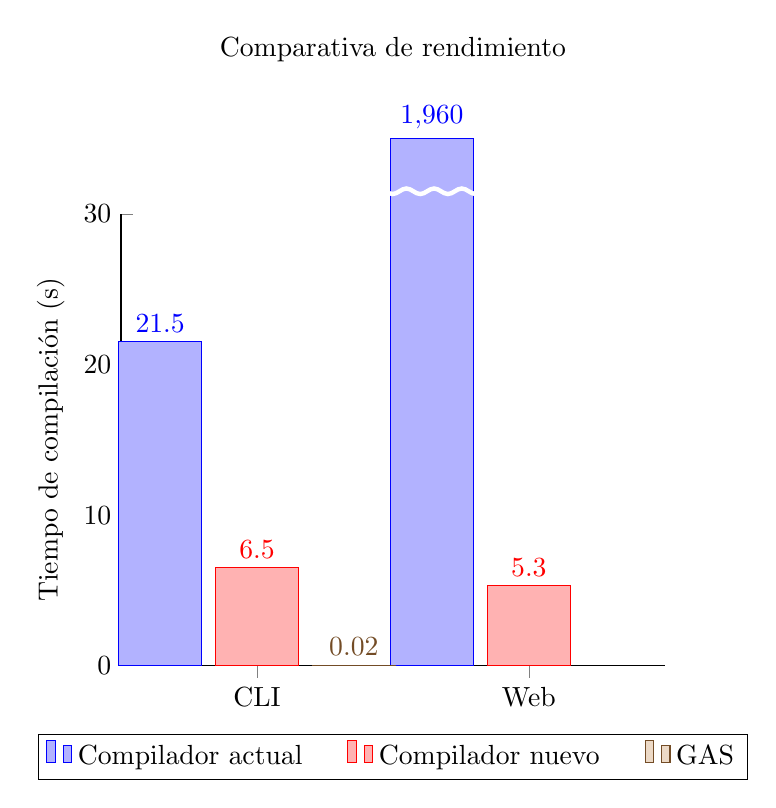
\begin{tikzpicture}
    \begin{axis}[
        width=0.7\textwidth,
        title={Comparativa de rendimiento},
        title style={yshift=1.6cm},
        ylabel={Tiempo de compilación (s)},
        symbolic x coords={\gls{CLI}, Web},
        xtick=data, % Fixes xticks appearing many times
        ybar=5pt, % Spacing between bars
        bar width=30pt,
        enlarge x limits=0.5, % Adds extra space at the sides
        legend style={ % Horizontal legend below the graph
            at={(0.5,-0.15)},
            anchor=north,
            legend columns=-1,
            /tikz/every even column/.append style={column sep=0.5cm}
        },
        axis lines*=left, % Add axes on the left and bottom
        every axis plot/.style={/pgf/number format/fixed},
        % Clip bars that are too high
        visualization depends on=rawy\as\rawy, % Save the unclipped values
        ymin=0, ymax=30, % Stop y axis at 30
        restrict y to domain*=0:35, % Cut values off at 35
        after end axis/.code={ % Add squiggly line for cutted graphs
            \draw[ultra thick, white, decoration={snake, amplitude=1pt}, decorate] (rel axis cs:0,1.05) -- (rel axis cs:1,1.05);
        },
        nodes near coords={\pgfmathprintnumber{\rawy}}, % Add the unclipped values
        clip=false, % Don't clip bars outside of the graph
    ]
        \addplot coordinates {(\gls{CLI}, 21.5)(Web,1960)};
        \addplot coordinates {(\gls{CLI}, 6.5)(Web,5.3)};
        \addplot coordinates {(\gls{CLI}, 0.02)(Web,nan)};
        \legend{Compilador actual,Compilador nuevo,GAS}
    \end{axis}
\end{tikzpicture}
}{rendimiento}{Comparativa de rendimiento entre los diferentes compiladores}
